% Released under CC-BY-SA 2012
% Author: Stefan Petersen <spe@ciellt.se> 
%
% This presentation is based on the conference-ornate-20min template
% by Till Tantau <tantau@users.sourceforge.net>.  You may redistribute
% and/or modify it under the terms of the GNU Public License, version
% 2.
%
% To produce a PDF from this document, do something like
%
%   pdflatex FILE.tex
%
% You might want to have packages like tetex, latex-beamer and
% ghostscript installed.

% Presentation (C) 2013, Stefan Petersen (spe(a)ciellt.se)
% Denna presentation är licenserad under Creative Commons BY-NC-SA 3.0
% Attribution-NonCommercial-ShareAlike
% http://creativecommons.org/licenses/by-nc-sa/3.0/

\documentclass{beamer}
\mode<presentation>
{
  \usetheme{Warsaw}
  \setbeamercovered{transparent}
}
\usepackage[english]{babel}
\usepackage[utf8]{inputenc}
\usepackage{times}
\usepackage[T1]{fontenc}
\usepackage{url}
\usepackage{cclicenses}
%%%%%%%%%%%%%%%%%%%%%%%%%%%%%%%%%%%%%%%%
\title{Grundläggande krypto och kryptering}
\subtitle{Krypto, kryptometoder och hur det hänger ihop}
\author{Stefan Petersen}
\date[2013-02-16]{Stockholm Crypto Party 2013 \\
  Released under Creative Commons BY-NC-SA 3.0 \\
  \cc \byncsa}
\pgfdeclareimage[height=0.5cm]{ndn-logo}{images/DFRI-logo}
\logo{\pgfuseimage{ndn-logo}}
%
%\AtBeginSection[]
%{
%  \begin{frame}<beamer>{Innehåll}
%    \tableofcontents[currentsection,currentsubsection]
%  \end{frame}
%}

% Enable this to make items appear one at a time.
%\beamerdefaultoverlayspecification{<+->}
%%%%%%%%%%%%%%%%%%%%%%%%%%%%%%%%%%%%%%%%
\begin{document}
\begin{frame}
  \titlepage
\end{frame}
\begin{frame}{Innehåll}
  \tableofcontents
\end{frame}
%%%%%%%%%%%%%%%%%%%%%%%%%%%%%%%%%%%%%%%%
\section{Presentation av mig}
\begin{frame}{Vem är jag?}
\begin{itemize}
\item Elektronikkonstruktör och programmerare
\item Eget företag sedan 2008, AB sedan 2012 (Ciellt AB)
\item Civilingenjör, Elektro, KTH, 1992-1998
\item Open source-projekt gerbv (gEDA) och sigrok
\item Krypto och kryptering eget intresse
\item Medlem i DFRI
\item Kontakt: spe@ciellt.se
\end{itemize}
\end{frame}
%%%%%%%%%%%%%%%%%%%%%%%%%%%%%%%%%%%%%%%%

%%%%%%%%%%%%%%%%%%%%%%%%%%%%%%%%%%%%%%%%
\section{Enkel binär matematik}

\begin{frame}{Enkel binär matematik}
\begin{itemize}
\item  Ett helt område inom matematiken för detta
\pause ==> Specialister, vilket jag inte är
\pause \item Militärt viktigt, många länder har stora hemliga avdelningar som 
bara sysslar med att analysera krypto (FRA, NSA, GCHQ)
\pause \item En siffra till i ett decimaltal ger 10 ggr fler kombinationer
\pause \item En bit till ger dubbelt så många kombinationer
\pause \item Bra att tänka på vid ``brute force''
\pause ==> öka ``bara'' antalet bitar
\end{itemize}
\end{frame}

\begin{frame}{Binär addition}
\begin{itemize}
\item Binär addition
\pause == exklusiv eller
\pause == exclusive or
\pause == exor
\pause \item En liten box med två ingångar och en utgång:\\
\pause 0 exor 0 => 0 \\
\pause 1 exor 0 => 1 \\
\pause 0 exor 1 => 1 \\
\pause 1 exor 1 => 0 \\
\pause \item Användes mycket i kryptona under andra världskriget och en bit in på 50-talet
\end{itemize}
\end{frame}

%%%%%%%%%%%%%%%%%%%%%%%%%%%%%%%%%%%%%%%%
\section{Kryptering med hemlig nyckel}

\begin{frame}{Hemlig nyckel}
\begin{itemize}
\item Både sändare och mottagare har samma nyckel för kryptering och dekryptering
\pause \item Måste ha kommit överens om nyckeln i förväg
\pause \item Delad hemlighet ==> ``shared secret''
\pause \item Om en av nycklarna ``läcker ut''  måste nya nycklar utbytas
\pause \item Oftast ganska enkelt att kryptera och dekryptera ==> ``lättviktigt'' 
\end{itemize}
\end{frame}

\begin{frame}{Exempel på krypto med hemlig nyckel}
\begin{itemize}
\item Substitutionskrypto (korsordskrypto)
\pause \item Enigma/Lorenz(Tunny)/Geheimfernschreiber
\pause \item DES (56 bitar)
\pause \item 3DES (56/112/168 bitar)
\pause \item AES (128/192/256 bitar)
\end{itemize}
\end{frame}

\begin{frame}{Enigma/Lorenz(Tunny)/Geheimfernschreiber}
\parbox{3.5cm}{\sloppy 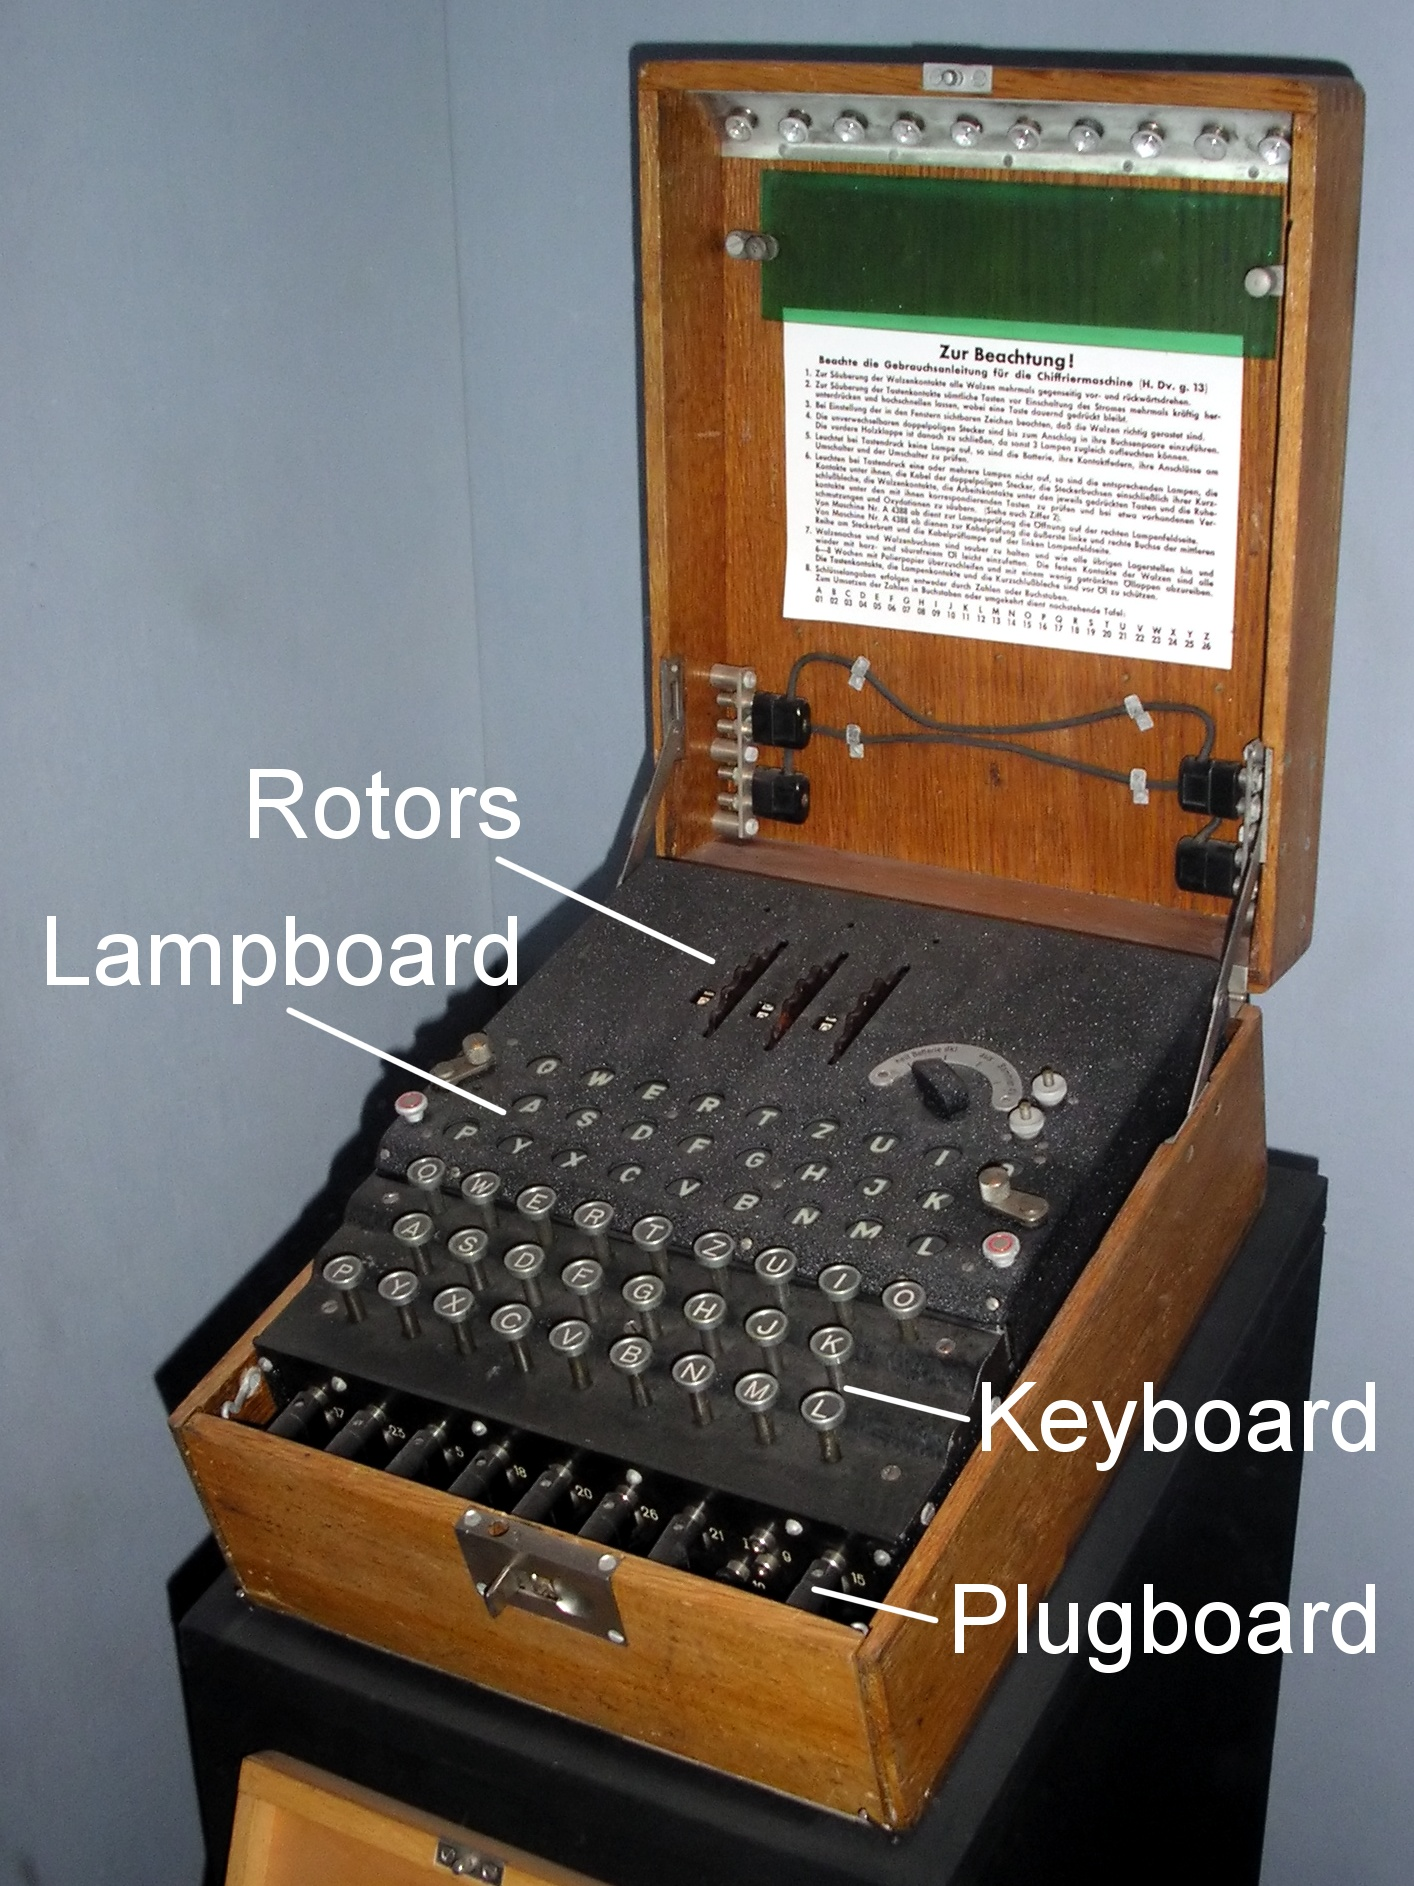
\includegraphics[width=3cm]{images/EnigmaMachineLabeled}}
\parbox{7cm}{\sloppy 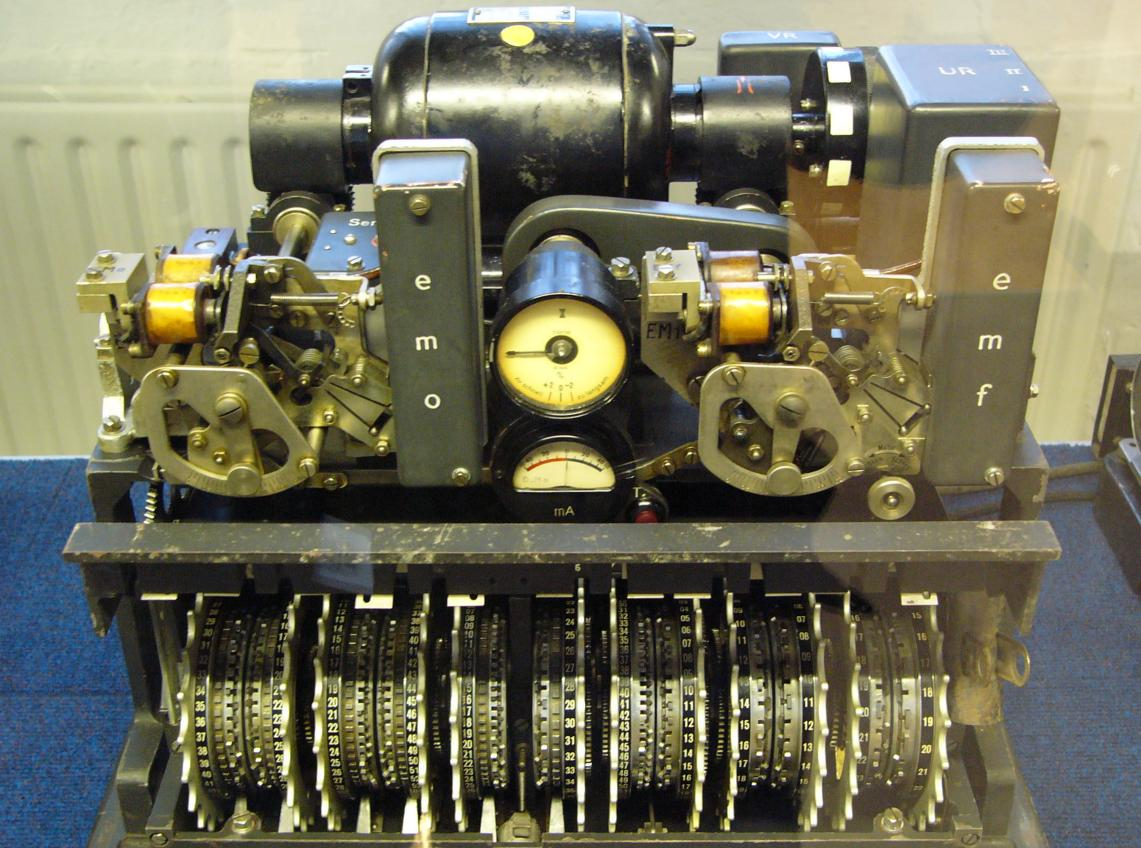
\includegraphics[width=7cm]{images/Lorenz-SZ42-2}}
\end{frame}

\begin{frame}{DES Data Encryption Standard}
\begin{itemize}
\item Var under många år  standardkryptot för t.ex. banker
\pause \item Publicerat 1977, standardiserades 1979
\pause \item Konstruktörer var IBM och då var nyckellängden 128 bitar (Lucifer)
\pause \item Efter att ha passerat igenom NSA var nyckellängden nere på 56 bitar
\pause \item EFF ``DES Cracker'' (Deep Crack) använder  ``brute force'' (1998)
\pause \item 3DES (triple DES) är egentligen DES tre gånger med olika nyckel
\pause \item (3 gånger med samma nyckel ger samma som DES 1 gång)
\end{itemize}
\end{frame}

\begin{frame}{Deep Crack}
\parbox{3.5cm}{\sloppy 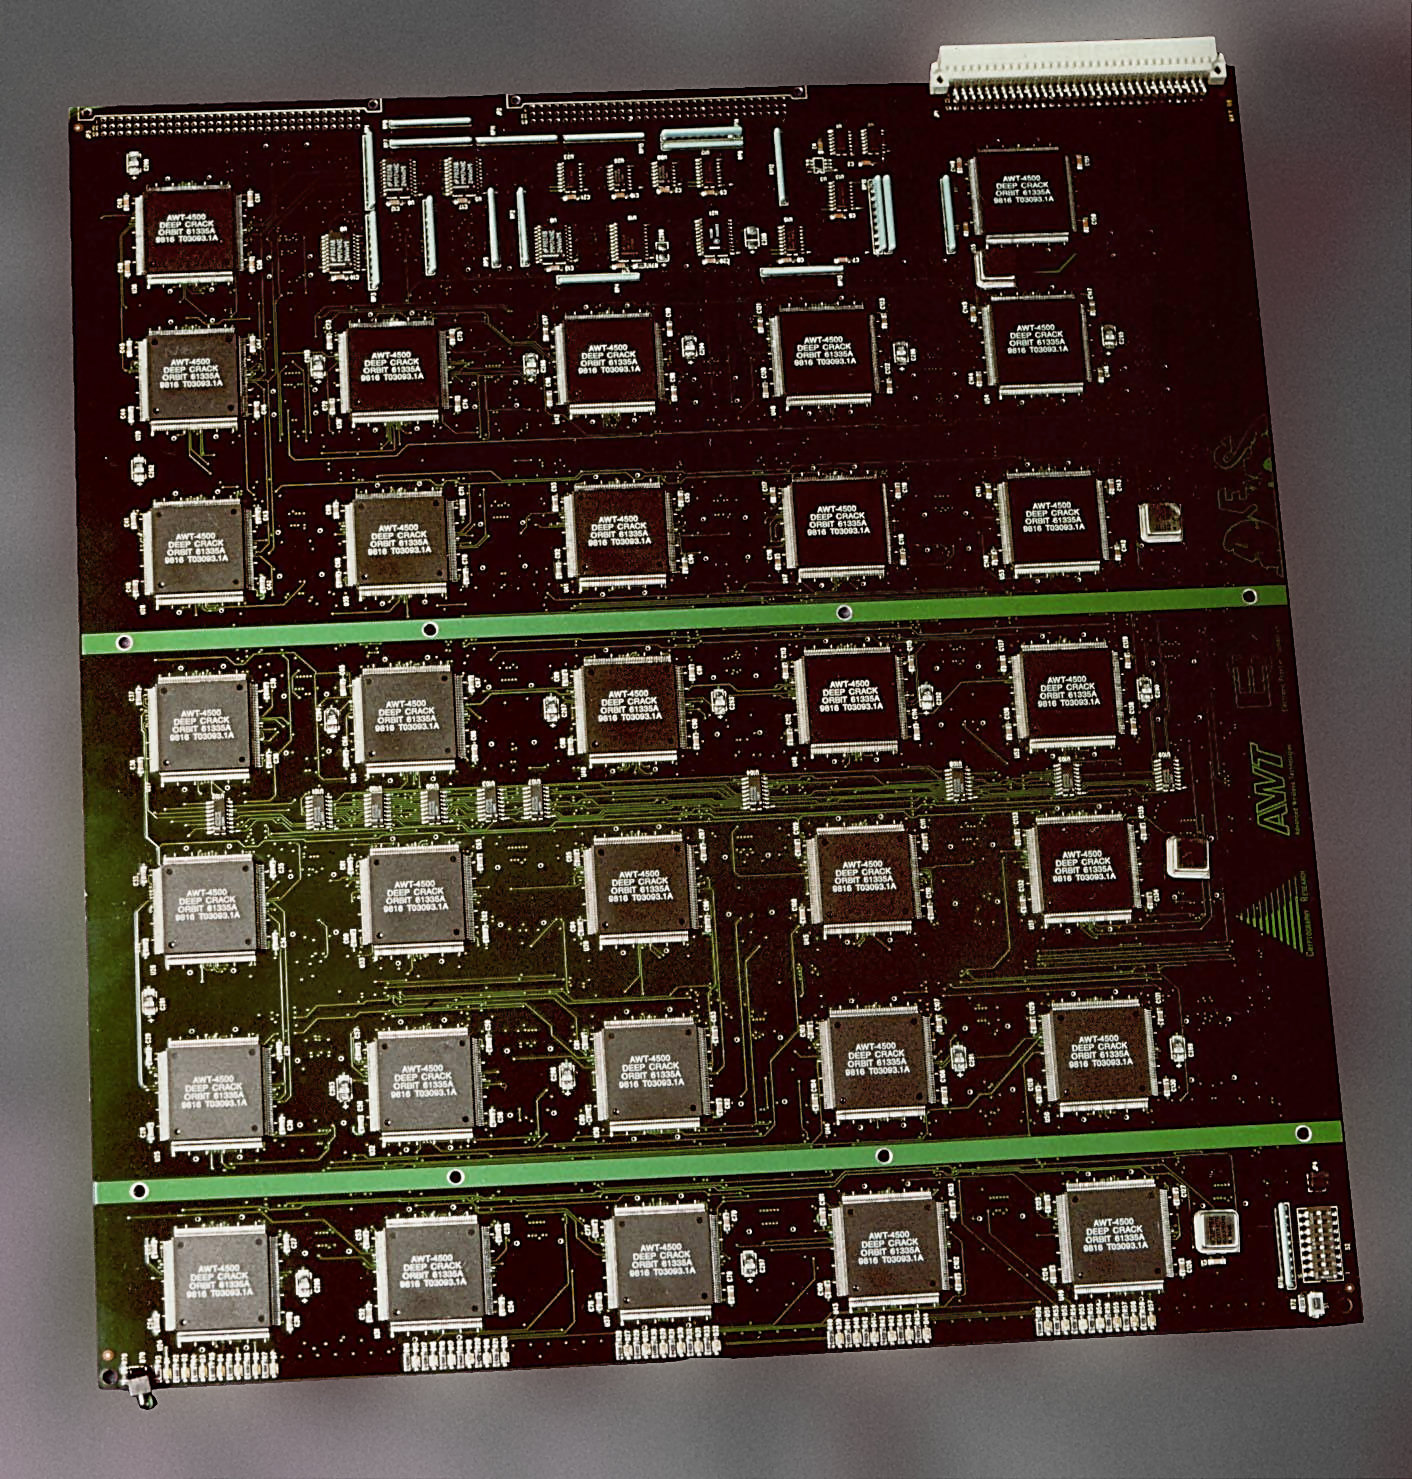
\includegraphics[width=3cm]{images/Board300}}
\parbox{7cm}{
EFF:s Deep Crack innehåller 1856 specialchips för att knäcka DES. Bilden visar ett 
dubbelsidigt kretskort från Deep Crack med 64 av dessa specialgjorda chips.
}
\end{frame}

\begin{frame}{AES Advanced Encryption Standard}
\begin{itemize}
\item Togs fram genom en öppen process
\pause \item NIST (National Institute of Standards \& Technology)
\pause \item 1997 annonserade NIST en ``skönhetstävling'' om vem som kunde ta fram en ersättare till DES
\pause \item Enkel att implementera i mjukvara och i hårdvara, säker, klara flera nyckellängder etc
\pause \item 15 förslag lämnades in
\pause \item Efter en process med flera konferenser, studier av varandras förslag etc kom NIST till ett avgörande
\pause \item 2000 beslutade NIST att utse ett förslag kallar Rijndael skulle bli AES
\pause \item Två holländare, Joan Daemen och Vincent Rijmen
\end{itemize}
\end{frame}


%%%%%%%%%%%%%%%%%%%%%%%%%%%%%%%%%%%%%%%%
\section{Kryptering med öppen nyckel}

\begin{frame}{Öppen nyckel}
\begin{itemize}
\pause \item Två nycklar, en publik (öppen) nyckel och en hemlig nyckel
\pause \item Publika nyckeln kan man dela ut till vem som helst
\pause \item Hemliga nyckeln måste man vakta väldigt hårt
\pause \item Komplicerad operation för en dator som tar lång tid
\pause \item Används oftast för att dela en hemlig nyckel med varandra för att sen fortsätta
med t.ex. AES
\end{itemize}
\end{frame}

\begin{frame}{Diffie-Hellman}
\begin{itemize}
\item 1976 föreslog Whitfield Diffie och Martin Hellman ett sätt att utbyta nycklar utan 
att tidigare delat en nyckel
\pause \item Malcolm J. Williamson, GCHQ , hade kommit på detta några år tidigare
\pause \item De kom på nyckelutbytesalgoritmen, men inte krypteringen
\end{itemize}
\end{frame}


\begin{frame}{RSA}
\begin{itemize}
\item Tre israeler 1977; Ron Rivest, Adi Shamir och Leonard Adleman (RSA)
\pause \item Patenterad fram tills den 20:e september, 2000
\pause \item Clifford Cocks, GCHQ, gjorde detta 1973, men vars arbete var klassificerat tills 1997.
\pause \item meddelande 
\pause ==> publik nyckel 
\pause ==> krypterat
\pause ==> hemlig nyckel 
\pause ==> meddelande
\end{itemize}
\end{frame}

\begin{frame}{Signering}
\begin{itemize}
\item Metoden går att köra "baklänges":
\pause \item meddelande 
\pause ==> hemlig nyckel 
\pause ==> krypterat
\pause ==> publik nyckel 
\pause ==> meddelande
\pause \item Signering
\pause \item nät-av-tillit (web-of-trust)
\pause \item Key Signing Party (senare i eftermiddag)
\end{itemize}
\end{frame}


\begin{frame}{Faktorisering}
\begin{itemize}
\item Båda nycklarna skapas ur två stora tal
\pause \item Om man från den publika nyckeln lyckas räkna ut vilka två stora tal den är 
skapad ur kan man skapa den hemliga nyckeln
\pause \item Faktoriseringsproblemet (``factoring problem'')
\pause \item Race mellan antal bitar i nyckeln och datorutvecklingen
\pause \item Eller att någon kommer på en smart lösning på faktoriseringsproblemet
\end{itemize} 
\end{frame}


%%%%%%%%%%%%%%%%%%%%%%%%%%%%%%%%%%%%%%%%
\section{Hashning}

\begin{frame}{Hash}
\begin{itemize}
\item Hashning är inte kryptering, kryptografisk hashning
\pause \item Hashning är att ur en stor massa med data skapa ett unikt fingeravtryck
\pause \item Minsta bit som ändras i datamassan ska skapa ett nytt fingeravtryck
\pause \item Man ska inte från en hash kunna återskapa datat (undvika kollisioner)
\pause \item Genom att jämföra den lokalt genererade hashen med den medskickade
hashen kan man se om någon har varit inne och ändrat i datat
\end{itemize}
\end{frame}

\begin{frame}{Kända algoritmer}
\begin{itemize}
\item MD2, MD4, MD5
\pause \item SHA-0, SHA-1, SHA-2 samt SHA-3 (finns fler)
\end{itemize}
\end{frame}

\begin{frame}{Användande}
\begin{itemize}
\item  Vanligast är MD5 samt SHA-1
\pause \item Fast båda är ``knäckta''
\pause \item Knäckt i hashningssammanhang innebär oftast att man kan finna kollisioner
``baklänges''
\pause \item MD-5 2008
\pause \item SHA-1 februari 2005 första attacken och i augusti 2005
\pause \item Tar fortfarande några hundra år att ``knäcka'', så det är nog lugnt ett tag till :)
\end{itemize}
\end{frame}

\begin{frame}{SHA-3}
\begin{itemize}
\item Standard under 2012
\pause \item Tävling precis som i AES
\pause \item Keccak var det vinnande bidraget
\pause \item Också holländare (en av dem från AES-tävlingen)
\pause \item Keccakpresentation på FOSDEM 2013
\end{itemize}
\end{frame}


%%%%%%%%%%%%%%%%%%%%%%%%%%%%%%%%%%%%%%%%
\section{Knäckning}

\begin{frame}{Knäckning}
\begin{center}
  När anses ett krypto knäckt?
\end{center}
\pause 
\begin{center}
  När det går fortare att använda knäckningsmetoden än ``brute force''
\end{center}
\pause 
\begin{center}
  Oftast betyder det att man gått från kanske tusentals år till hundratals år
\end{center}
\pause 
\begin{center}
  Men mycket beror ju på hur länge man vill att det ska vara hemligt
\end{center}
\end{frame}

\begin{frame}{Kända sätt att attackera krypton}
\begin{itemize}
\item  Frekvensanalys
\pause \item Klartextjämförelse
\pause \item Rå styrka ("brute force")
\pause \item Fel i implementationer
\pause \item Matematiska bevis
\end{itemize}
\end{frame}

\begin{frame}{Frekvensanalys}
\begin{itemize}
\item  substitutionskrypto, byt bokstav mot bokstav ("korsordskrypto")
\pause \item För svenska: E A T R S...
\pause \item https://sv.wikipedia.org/wiki/Bokstavsfrekvens
\pause \item Även kända ord, typiskt med dubbla t:n: ``att'', ``hitta'', ``skatt''...
\end{itemize}
\end{frame}

\begin{frame}{Klartextjämförelse}
\begin{center}
Enigma/Lorenz/Geheimfernschreiber
\end{center}
\begin{center}
Enligt uppgift knäcktes dessa chiffer genom att slarviga operatörer först sände
meddelandet okrypterat, sedan samma meddelande krypterat.
\end{center}
\end{frame}

\begin{frame}{GSM-krypto}
\begin{itemize}
\item Chaos Computer Congress 2010 visade Karsten Nohl och Sylvain Munaut 
  ``live'' hur man kunde lyssna på GSM-trafik
\pause \item Alla paket som sänds är lika stora
\pause \item Ett ACK-paket är 1-3 byte, resten är ``skräp''
\pause \item ``Skräpet'' är alltid likadant
\pause \item Därför kan man räkna ut nyckeln baklänges (``rainbow tables'')
\pause \item Samma nyckel används i flera transaktioner
\pause \item https://gsmmap.org
\end{itemize}
\end{frame}

\begin{frame}{Rå styrka}
\begin{center}
\parbox{6cm}{\sloppy 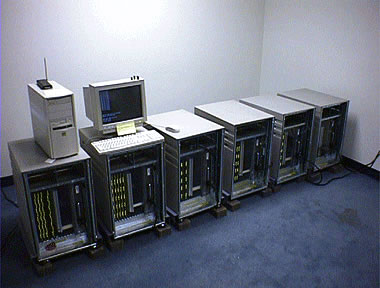
\includegraphics[width=6cm]{images/DES-machine}\\
\tiny{EFF:s "Deep Crack"}}
\parbox{6cm}{ \sloppy
\begin{center}
 ``Prova alla kombinationer''
\end{center}}
\end{center}
\end{frame}

\begin{frame}{Fel i implementationer}
\begin{itemize}
\pause \item Mozilla, slumptal begränsade till 16 bitar
\pause \item Mifare Classic, eget krypto
\pause \item Mifare Classic, slumptalsgeneratorn startar alltid på noll
\pause \item GSM, eget krypto
\end{itemize}
\end{frame}

\begin{frame}{Matematiska bevis}
\begin{center}
\pause
Detta är ett helt eget fält inom matematiken som iallafall är bortom min förståelse.
\end{center}
\end{frame}


%%%%%%%%%%%%%%%%%%%%%%%%%%%%%%%%%%%%%%%%

\section{Avslutning}

\begin{frame}{Slutsats}
\begin{itemize}
\item Implementera aldrig ett eget krypto: \\
\pause  -- Matematiskt \\
\pause  -- Programatiskt
\pause \item Leta efter begränsningar i implementationen
\pause \item Publicera din lösning
\end{itemize}
\end{frame}


\begin{frame}{Källor}
\begin{itemize}
\item Wikipedia har ett stort sortiment av bra artiklar i detta ämne
\pause \item ``Crypto'', Steven Levy,
\pause \item ``Kodboken'' (``The Code Book''), Simon Singh
\pause \item ``Svenska kryptobedrifter'', Bengt Beckman
\pause \item ``Applied Cryptography'', Bruce Schneier
\end{itemize}
\end{frame}

\begin{frame}{Frågor}
\begin{center}
TACK!\\
Frågor?
\end{center}
\end{frame}


%%%%
\end{document}
